%!TEX root = ../report.tex

\section{Symmetric Cryptography}
In symmetric encryption two communication partners Alice and Bob share a secret key that is used for encryption and decryption.
It ensures only confidentiality, not integrity or authenticity.\\

We use the following terminology:
\begin{itemize}[noitemsep, topsep=0pt]
  \item Key $k$
  \item Plaintext $m = Dec_k(c)$
  \item Ciphertext $c = Enc_k(m)$
  \item $Dec_k(Enc_k(m)) = m$
\end{itemize}

\subsection{One-Time-Pad (OTP): A Perfect Cypher}
For the OTP a perfectly random bitstream opt with the length of the message to encode is needed.
Then the encryption operation is defined as $Enc_{otp}(m) = m \oplus otp$ and the decryption operation as $Dec_{otp}(c) = c \oplus otp$
For the OTP to be perfectly secure, the key must only be used once which is impractical in the real world where we usually want $length(k) \ll length(m)$ and thus reusable keys.

\subsection{Security of Cyphers}
Kerckhoff's principle states that the cipher method must not be required to be secret, and it must be able to fall into the hands of the enemy without inconvenience.
Thus only the key needs to be secret.\\
It is advisable to use only standardized ciphers from libraries and RTFM (read the fucking manual) because implementing own ciphers has a lot of pitfalls and is more often or almost always done wrong.
Furthermore encryption does not imply that the system is secure, often integrity and authenticity is more important than confidentiality.
And also do not forget key management.

\subsection{Attacking Symmetric Ciphers}
The goals of attacks on ciphers is to learn something about m given a c.
Getting any information about k from an attack is also considered a successful one.\\

Possible attack scenarios are:
\begin{itemize}[noitemsep, topsep=0pt]
  \item Ciphertext-only-attack: attacker knows c
  \item Known-plaintext-attack: For a fixed k, the attacker got a pair (m, c) and tries to learn something about other ciphertexts
  \item Chosen-plaintext and chosen-ciphertext attack: similar to previous attack, but attacker can chose m or c freely
\end{itemize}
\vspace{10pt}

A cipher is secure if the best known attack is brute-forcing all keys.

\subsection{Block and Stream Ciphers}
A block cipher encrypts and decrypts inputs of length n to outputs of length n ($\Rightarrow$ block length n).
A steam cipher on the other hand generates a random bitstream with arbitrary length, called keystream, that is xored to the plain text to encrypt and decrypt.\\
The most advisable cipher to use is probably the AES block cipher.
It is well tested and proven to be (mostly) secure and hardware supported what makes it quite fast ($>2GB/s$ with HW support, $200Mbit/s$ without).

\subsection{Modes of Encryption}
Modes of encryption are necessary to handle messages of variable length with block ciphers.
The plaintext therefore is split into parts of length equal to the cipher block length.
If the last block is shorter than the block length, we add padding.

\subsection{Electronic Code Book Mode (ECB)}
\begin{figure}[H]
  \centering
  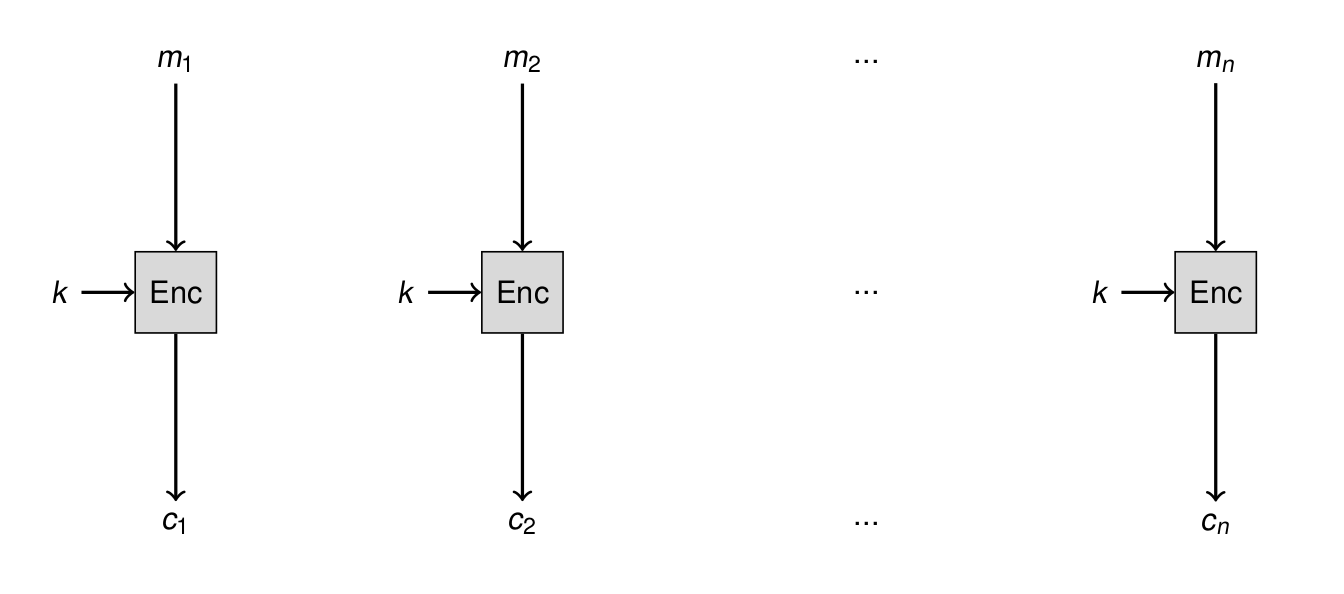
\includegraphics[width=.8\textwidth]{figures/ecb.png}
\end{figure}
In ECB, every plaintext block is encrypted with the unmodified key as input.
The problem thereby is that identical plaintext blocks result in the same ciphertext blocks.
\begin{figure}[H]
  \centering
  
\includegraphics[width=.8\textwidth]{figures/ecb_problem.png}
\end{figure}

\subsection{Cipher Block Chaining Mode (CBC)}
\begin{figure}[H]
  \centering
  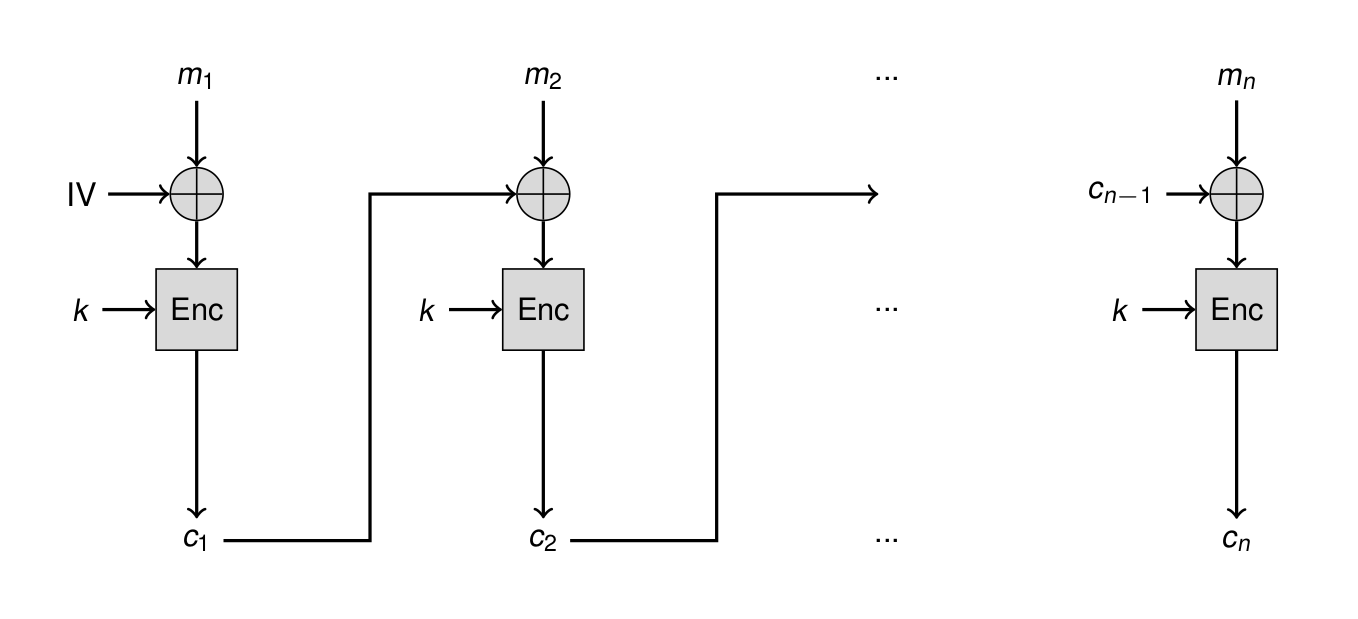
\includegraphics[width=.8\textwidth]{figures/cbc_encrypt.png}
  \caption{CBC Encrypt}
\end{figure}
CBC uses the ciphertext from the previous block xored with the current message block and the unmodified key k as inputs of the encryption function $c_i = Enc_k(c_{i-1} \oplus m_i)$.
For the first message, where no previous cipher block is available, an initialization vector (IV) is used which may be sent in plaintext and is fresh for every massage (or packet if the message is split across multiple packets).\\
Compared to ECB, the advantage is that equal plaintext blocks/messages are not encrypted to the same ciphertext blocks/messages.
\begin{figure}[H]
  \centering
  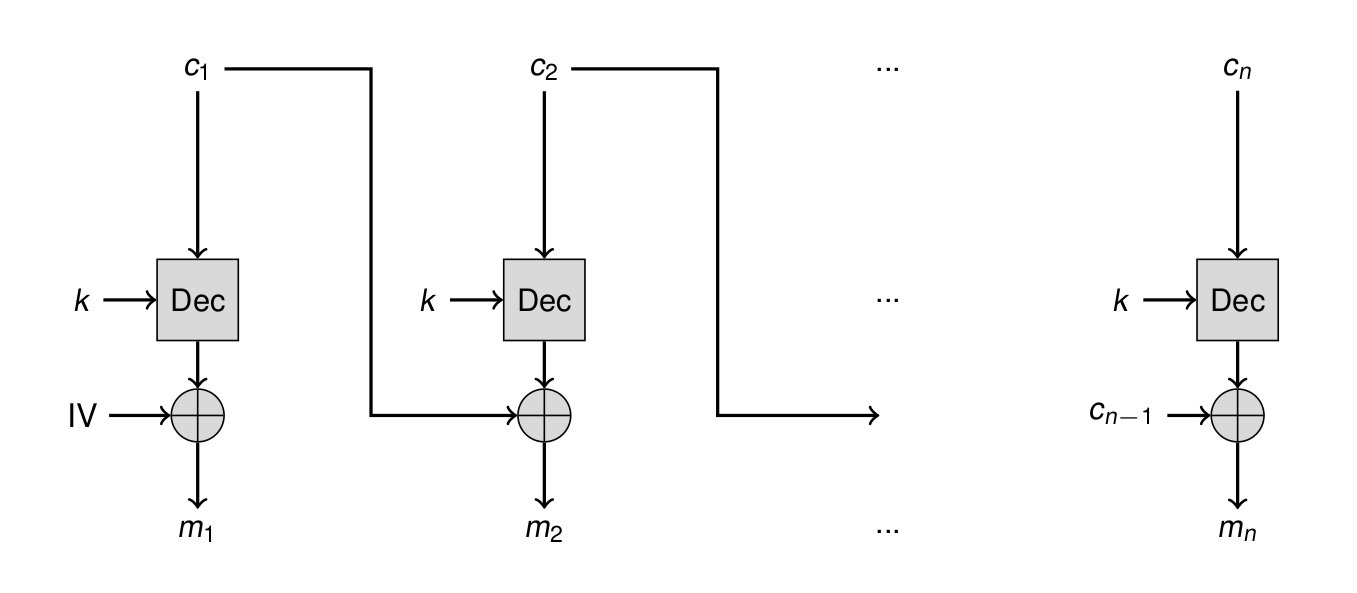
\includegraphics[width=.8\textwidth]{figures/cbc_decrypt.png}
  \caption{CBC Decrypt}
\end{figure}
Decryption is defined by $m_i = c_{i-1} \oplus Dec_k(c_i)$.

\subsection{Output Feedback Mode (OFB)}
\begin{figure}[H]
  \centering
  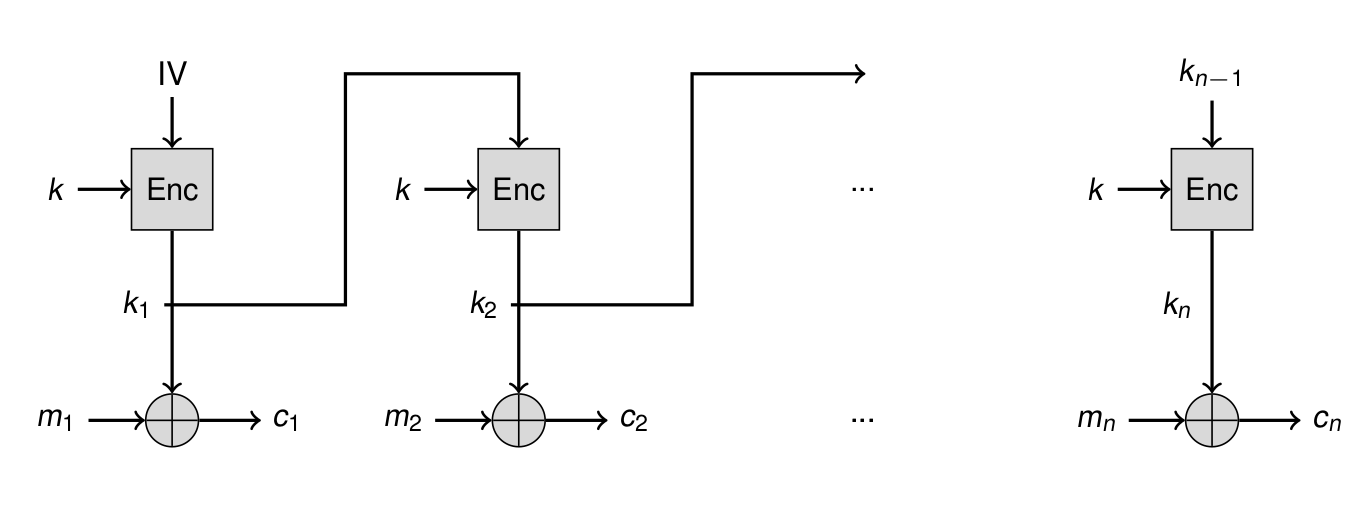
\includegraphics[width=.8\textwidth]{figures/ofb_encrypt.png}
  \caption{OFB Encrypt}
\end{figure}
OFB transforms a block cipher into a stream cipher.
In step $i$, it takes cipher key $k_{i-1}$ form the previous step and encrypts it with the key k.
This cipher key $k_i$ is then xored with the corresponding plaintext block $m_i$ to calculate the ciphertext $c_i$.
In the first step an IV is used as $k_{i-1}$.

\begin{figure}[H]
  \centering
  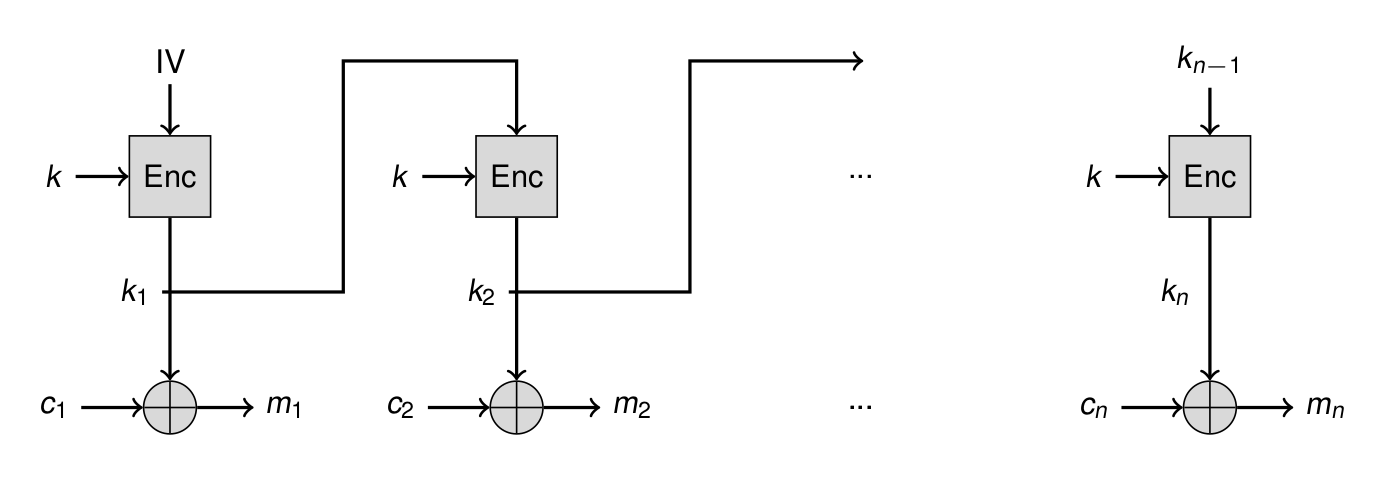
\includegraphics[width=.8\textwidth]{figures/ofb_decrypt}
  \caption{OFB Decrypt}
\end{figure}
Decryption is the same procedure except that the key stream is xored with the cipher text blocks.
\newpage

\subsection{Counter Mode (CTR)}
\begin{figure}[H]
  \centering
  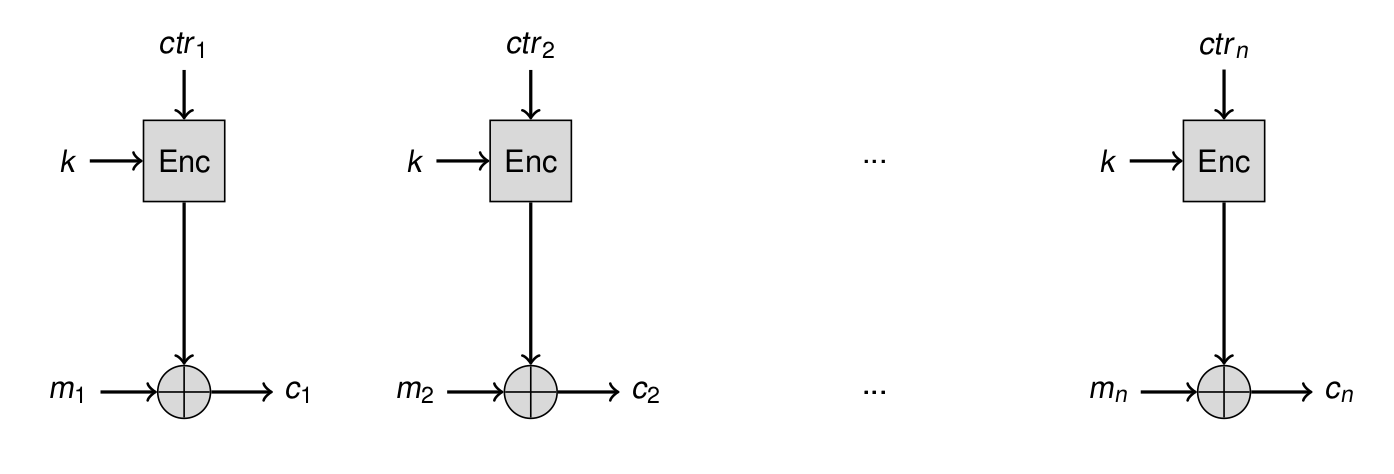
\includegraphics[width=.8\textwidth]{figures/ctr_encrypt}
  \caption{CTR Encrypt}
\end{figure}
In step $i$, CTR encrypts a counter $ctr_i = IV || i$ with key k and xors the result with the plaintext block $m_i$.
Like OFB, CTR also transforms block ciphers into stream ciphers.

\begin{figure}[H]
  \centering
  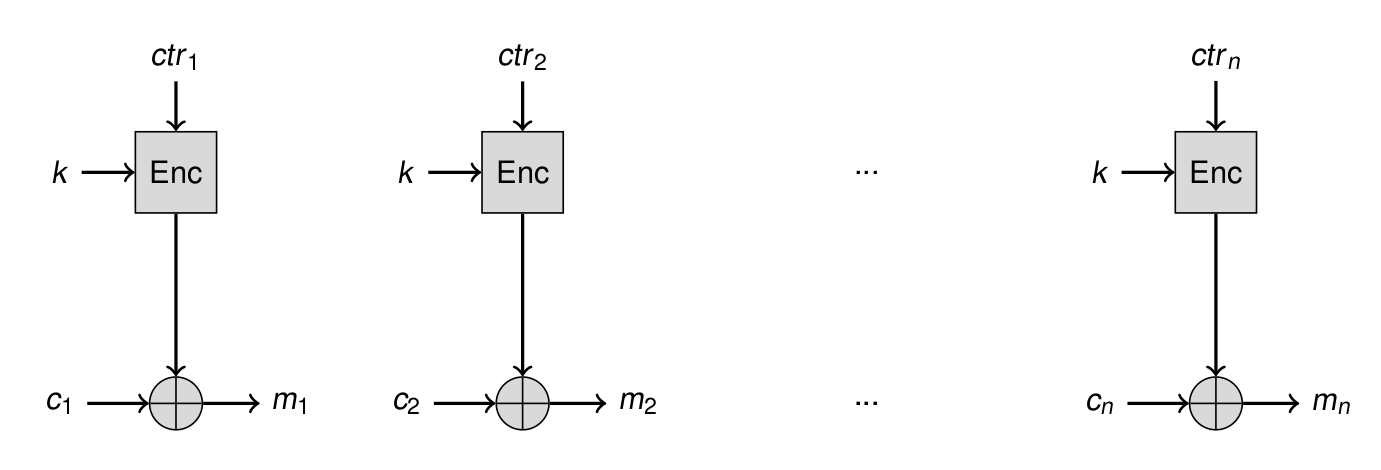
\includegraphics[width=.8\textwidth]{figures/ctr_decrypt.png}
  \caption{CTR Decrypt}
\end{figure}
Decryption is done by $m_i = Enc_k(ctr_i) \oplus c_i$.
